\documentclass[tikz]{standalone}
\usetikzlibrary{arrows.meta}
\begin{document}

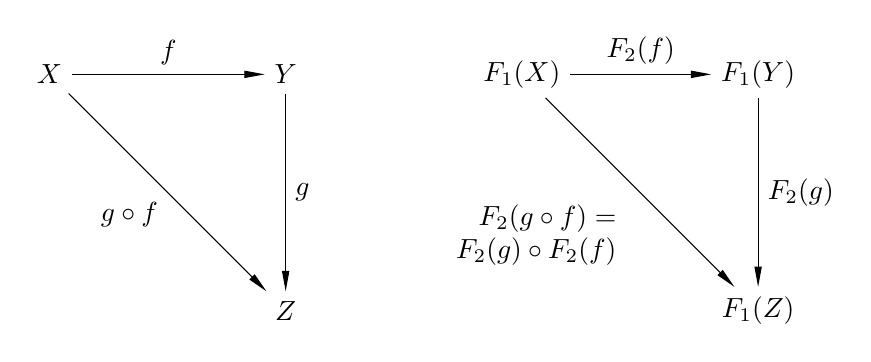
\begin{tikzpicture}[-latex, arrows={-Triangle[angle=20:5pt,scale=1.5]}]
	\node (X) at (0,0) {\(X\)};
	\node (Y) at (3,0) {\(Y\)};
	\node (Z) at (3,-3) {\(Z\)};
	\draw (X) to node [above] {\(f\)} (Y);
	\draw (Y) to node [right] {\(g\)} (Z);
	\draw (X) to node [below left] {\(g \circ f\)} (Z);

	\begin{scope}[xshift=6cm]
		\node (FX) at (0,0)  {\(F_1(X)\)};
		\node (FY) at (3,0)  {\(F_1(Y)\)};
		\node (FZ) at (3,-3) {\(F_1(Z)\)};
		\draw (FX) to node [above] {\(F_2(f)\)} (FY);
		\draw (FY) to node [right] {\(F_2(g)\)} (FZ);
		\draw (FX) to node [below left] 
		{\(\begin{array}{r}
			F_2(g \circ f) = \\ 
			F_2(g) \circ F_2(f)
		\end{array}\)} (FZ);
	\end{scope}
\end{tikzpicture}

\end{document}
